BriefCASE provides access to two analysis tools (GearCASE~\cite{gearcase2020} and
DCRYPPS~\cite{dcrypps2019}) that can examine AADL models to detect potential cyber vulnerabilities
and suggest requirements for mitigation.
%
Systems engineers are then presented with a requirements management interface
(Figure~\ref{fig:req-mgmt}) for viewing the generated requirements and importing them into the model
so they can be addressed. The interface enables engineers to select the requirements they wish to
import and assign them unique identifiers, or omit them with rationale. A document listing the omitted
requirements and rationale is maintained and may be a required development artifact for some
certification domains. 

\begin{figure*}[h]
	\centering
	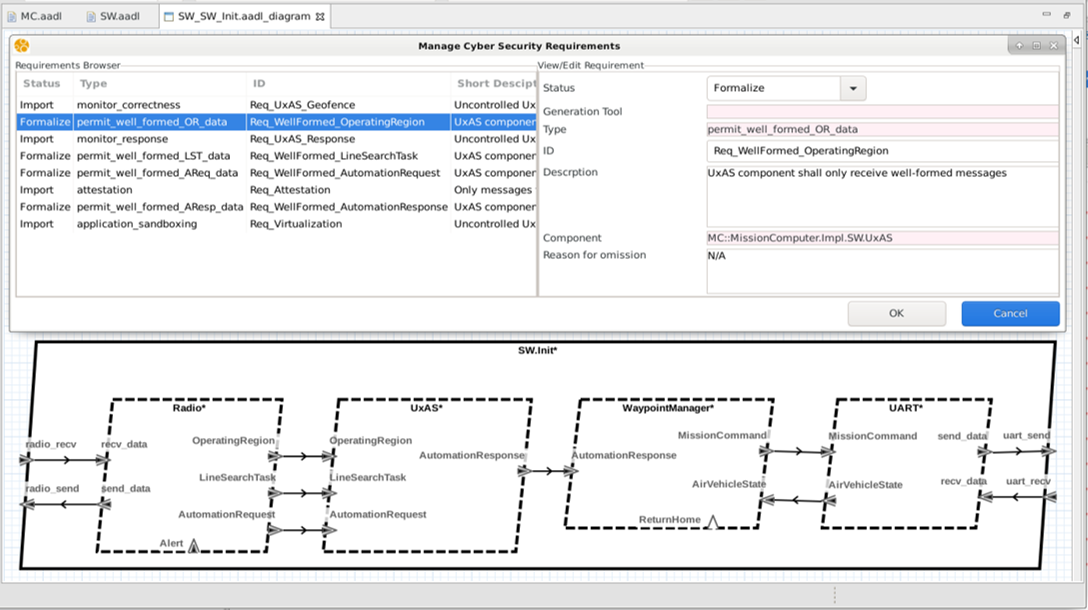
\includegraphics[width=0.8\textwidth]{figs/req-mgmt.png}
	\caption{Requirements management interface.  IS THIS FIG NEEDED?} 
	\label{fig:req-mgmt} 
\end{figure*}

Some requirements can also be formalized as assume-guarantee contracts
added to the AADL model, enabling formal verification. 
Such a requirement will be imported into the model with with an associated formal
contract.

A BriefCASE project contains a repository for requirements. Imported requirements are represented 
as assurance case goals to be satisfied. For example, one of the requirements for well-formedness 
messages selected in \figref{fig:req-mgmt} is imported as the goal shown in \figref{fig:req-wellformed-or}.
Initially, the goal is marked {\em undeveloped} and does not contain any evidential statements.  
These will be added as the design is updated to address this requirement.  
%for Resolute to evaluate in order to determine whether the goal has been satisfied. Running Resolute
%at this time will therefore produce a failed assurance case.

\begin{figure}[h]
	\centering
	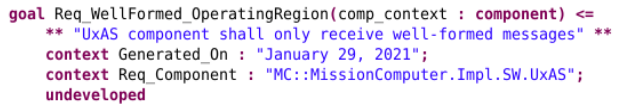
\includegraphics[width=1\columnwidth]{figs/req-wellformed-or.png}
	\caption{Requirement for well-formed messages.  NEEDED? CONVERT TO TEXT?} 
	\label{fig:req-wellformed-or} 
\end{figure}